%%%%%%%%%%%%%%%%%%%%%%%%%%%%% Define Article %%%%%%%%%%%%%%%%%%%%%%%%%%%%%%%%%%
\documentclass{article}
%%%%%%%%%%%%%%%%%%%%%%%%%%%%%%%%%%%%%%%%%%%%%%%%%%%%%%%%%%%%%%%%%%%%%%%%%%%%%%%

%%%%%%%%%%%%%%%%%%%%%%%%%%%%% Using Packages %%%%%%%%%%%%%%%%%%%%%%%%%%%%%%%%%%
\usepackage{listings, xcolor}
\usepackage{parskip}
\usepackage{hyperref}
\usepackage{amsmath}
\usepackage{graphicx}
\usepackage[a4paper, margin = 1.5cm]{geometry}
\usepackage{float}
\usepackage{amssymb}

%%%%%%%%%%%%%%%%%%%%%%%%%%%%%%% Title & Author %%%%%%%%%%%%%%%%%%%%%%%%%%%%%%%%
\title{Diagrammi di Sequenza}
\author{Trentin Tommaso}
%%%%%%%%%%%%%%%%%%%%%%%%%%%%%%%%%%%%%%%%%%%%%%%%%%%%%%%%%%%%%%%%%%%%%%%%%%%%%%%

\begin{document}
  \maketitle
  \tableofcontents
  \newpage

  \section{Diagrammi UML Comportamentali}
    Diagrammi che modellano comportamento dinamico degli elementi che compongono un sistema.
  \section{Diagrammi di Interazione}
    Diagrammi che modellano \textbf{collaborazione dinamica} tra oggetti che collettivamente implementano un determinato comportamento.
  \section{Diagrammi di Sequenza - Notazione}
    \subsection{Diagramma di Sequenza}
      Modella interazioni tra 1+ attori e le parti del sistema SW, nell'ambito dell'esecuzione di uno o più scenari di un caso d'uso:
      \begin{itemize}
        \item Interazioni tra \textbf{attori} e \textbf{oggetti} del sistema sono modellate in forma di \textbf{messaggi} (OO paradigm); 
        \item Scambio di messaggi viene letto dall'alto al basso;
        \item Chiariscono chiamate tra partecipanti e responsabilità di ciascuno di loro.
      \end{itemize}
    \subsection{Attore}
      \begin{itemize}
        \item Rappresentati come nel diagramma dei casi d'uso; 
        \item Riportati a sinistra con frecce che modellano interazioni verso gli oggetti del sistema;
        \item Possono non essere presenti nel caso uno scenario venga avviato da un altro scenario o dal sistema stesso.
      \end{itemize}
      \begin{figure}[h!]
        \begin{center}
          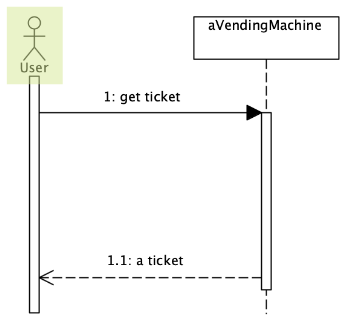
\includegraphics[width=0.3\textwidth]{figures/ds_act.png}
        \end{center}
      \end{figure} 
    \subsection{Partecipante / Istanza di classe}
      Istanze delle classi rappresentate da rettangoli etichettati in uno dei seguenti modi:
      \begin{itemize}
        \item con nome della classe e identificatore dell'oggetto nel formato \textbf{nomeOggetto:nomeClasse};
        \item con nome che suggerisce che si considera un'istanza di una classe (anOrder, aProduct...). 
      \end{itemize}
      \begin{figure}[h!]
        \begin{center}
          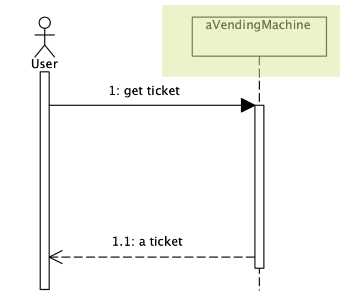
\includegraphics[width=0.3\textwidth]{figures/ds_ins.png}
        \end{center}
      \end{figure}
    \subsection{Lifeline}
      Mostrano i partecipanti mediante linea verticale tratteggiata dall'alto in basso che parte dai partecipanti, ne rappresentano il periodo temporale di vita (mostrano ordinamento messaggi, non durata temporale interazione!).
      \begin{figure}[h!]
        \begin{center}
          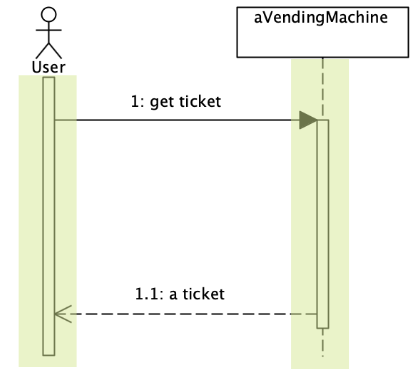
\includegraphics[width=0.3\textwidth]{figures/ds_ll.png}
        \end{center}
      \end{figure}
    \subsection{Messaggio}
      \begin{itemize}
        \item Definisce particolare comunicazione tra le lifeline di un'interazione; 
        \item Rappresentato mediante freccia tra lifeline (attore / oggetto o oggetto / oggetto);
        \item Ordine dei messaggi ricalca ordine sequenziale con il quale essi vengono scambiati.
      \end{itemize}
      \begin{figure}[h!]
        \begin{center}
          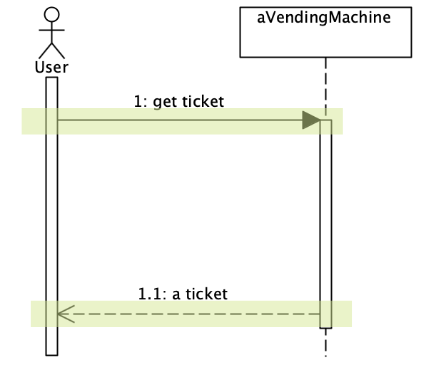
\includegraphics[width=0.3\textwidth]{figures/ds_msg.png}
        \end{center}
      \end{figure}

      \subsubsection{Scambio di Messaggi}
        Un messaggio può:
        \begin{itemize}
          \item Invocare operazione (\textbf{chiamata}); 
          \item Creare / distruggere istanza;
          \item Inviare segnale / dato.
        \end{itemize}
        I messaggi possono invocare operazioni in modo sincrono / asincrono e, quando lifeline riceve messaggio di chiamata, deve esistere \textbf{corrispondente operazione nella classe della lifeline ricevente}.
      \subsubsection{Tipi}
        \begin{figure}[h!]
          \begin{center}
            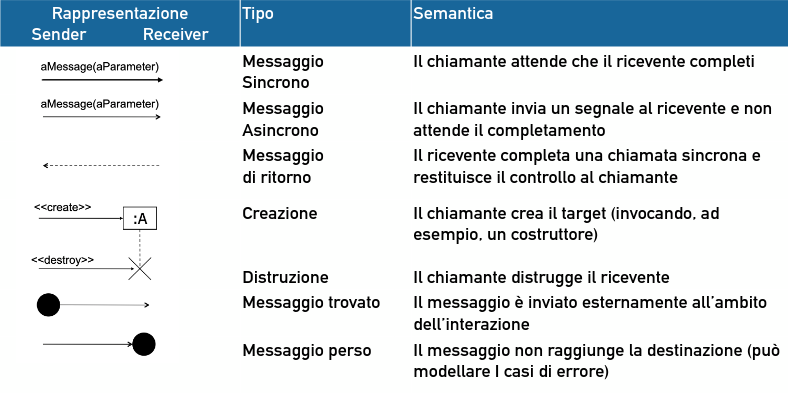
\includegraphics[width=0.5\textwidth]{figures/msg_type.png}
          \end{center}
        \end{figure}
    \subsection{Activation Box}
      Rettangoli che coprono parte delle lifeline, rappresentano periodo in cui istanza è attiva nell'interazione. Lifeline di un partecipante si attiva quando esso elabora un messaggio: durante esecuzione l'attivazione si sposta tra le lifeline descrivendo flusso di controllo.
      \begin{figure}[h!]
        \begin{center}
          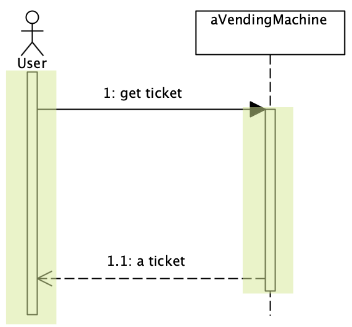
\includegraphics[width=0.3\textwidth]{figures/ds_ab.png}
        \end{center}
      \end{figure}
    \subsection{Messaggi di auto-delega / Activation box innestate}
      Auto-delega o chiamata interna quando un oggetto invia un messaggio a se stesso (chiamata a proprio metodo), ciò genera un'attivazione innestata. 
      \begin{figure}[h!]
        \begin{center}
          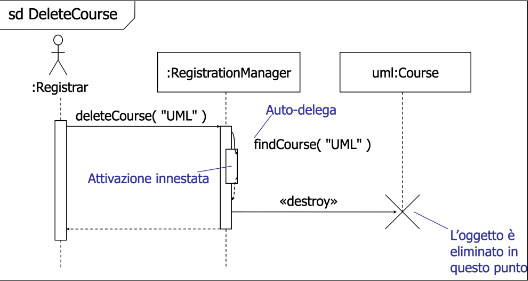
\includegraphics[width=0.5\textwidth]{figures/ds_ad.png}
        \end{center}
      \end{figure}
  \section{Dagli Scenari ai Diagrammi di sequenza al Codice OO}
    Vedi esempio da slide 16 su 10_sequence_diagrams.pdf
  \section{Paradigmi di Modellazione Centralizzati / Distribuiti}
    \noindent
    \begin{minipage}[t]{0.48\textwidth}
      \textbf{Centralizzato}: un singolo oggetto ha controllo, gli altri forniscono servizi.
      \begin{itemize}
        \item \textbf{Pro}: semplice soluzione che tende a raccogliere in un solo punto tutta l'elaborazione.
        \item \textbf{Contro}: logica che gestisce attributi potrebbe trovarsi in classi diverse, rendendo manutenzione non intuitiva.
      \end{itemize}
      \vspace{0.5cm}
      \centering
      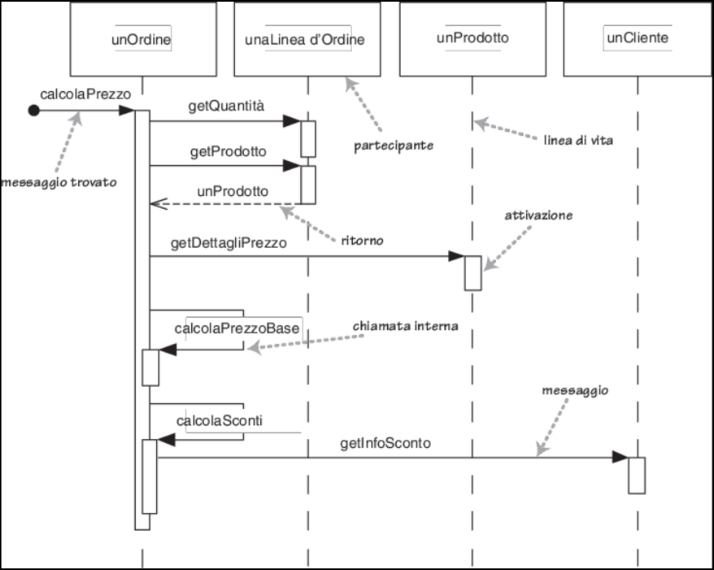
\includegraphics[width=0.75\linewidth]{figures/par_centr} 
    \end{minipage}
    \hfill
    \begin{minipage}[t]{0.48\textwidth}
      \textbf{Distribuito}: responsabilità distribuite tra gli oggetti partecipanti.
      \begin{itemize}
        \item \textbf{Pro}: conforme a paradigma OO, facilita manutenzione raccogliendo nello stesso oggetto dati / logica che potrebbero essere modificati assieme (permette utilizzo polimorfismo al posto di logica condizionale).
        \item \textbf{Contro}: può risultare dispersivo / difficile da leggere durante l'analisi.
      \end{itemize}
      \vspace{0.5cm}
      \centering
      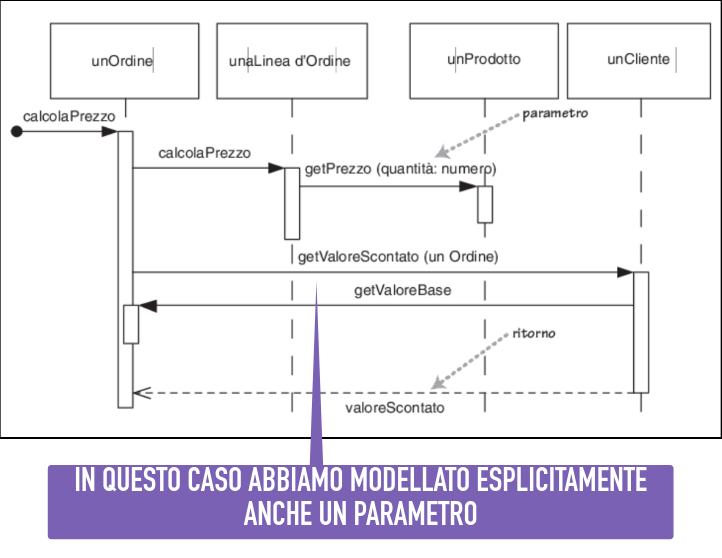
\includegraphics[width=0.75\linewidth]{figures/par_distr}
    \end{minipage}
  \section{Creazione / Distruzione degli Oggetti}
    \subsection{Creazione}
      Un messaggio al costruttore (etichettato come \textbf{new}) di un oggetto può creare un oggetto che viene disegnato al termine della freccia corrispondente al messaggio. Oggetti staticamente definiti partono dalla cima del diagramma e, in caso il partecipante faccia qualcosa appena creato, la activation box si disegna attaccata al rettangolo.
    \subsection{Distruzione}
      Se freccia del messaggio tra oggetti termina con una X allora oggetto che invia il messaggio sta distruggendo quello che lo riceve, una X alla fine della lifeline, senza messaggio, indica che l'oggetto sta distruggendo se stesso. Una volta distrutto un oggetto non è puù disponibile per l'elaborazione. 
    \begin{figure}[h!]
      \begin{center}
        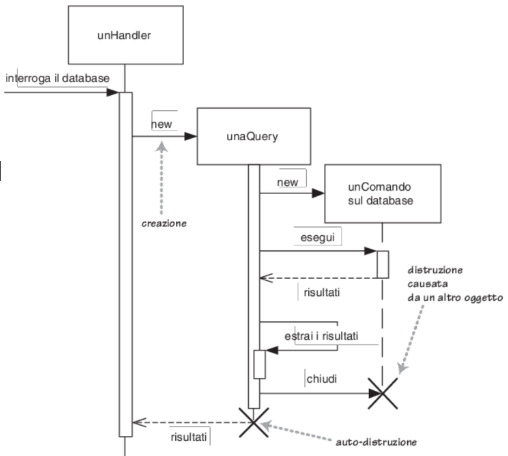
\includegraphics[width=0.3\textwidth]{figures/cre_dis.png}
      \end{center}
    \end{figure}
  \section{Frame di interazione / Frammenti combinati}
    \subsection{Limitazioni notazione base}
      \begin{itemize}
        \item Diagrammi di sequenza sono più adatti a descrivere interazione tra oggetti che la logica di controllo; 
        \item Notazione base non permette di rappresentare comportamenti ciclici / condizionali;
        \item UML2 implementa frame e frammenti con i loro operatori per ovviare a questi limiti.
      \end{itemize}
    \subsection{Idea}
      Frame di interazione evidenziano una parte del diagramma e racchiudono sottosequenza di messaggi, possono essere composti da 1+ frammenti combinati. Ogni frame ha:
      \begin{itemize}
        \item \textbf{1 operatore} che determina come vengono eseguiti suoi operandi; 
        \item \textbf{1+ frammenti};
        \item \textbf{0+ condizioni di guardia} che stabiliscono se frammenti corrispondenti devono essere eseguiti
      \end{itemize}
    \subsection{Operatori frammento più usati}
      \begin{figure}[h!]
        \begin{center}
          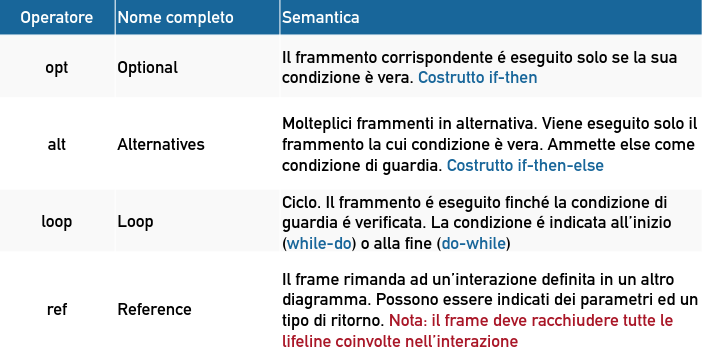
\includegraphics[width=0.5\textwidth]{figures/fra_mu.png}
        \end{center}
      \end{figure}
    \subsection{Pro e Contro}
      \begin{itemize}
        \item \textbf{Pro}:
          \begin{itemize}
            \item permettono di rappresentare costrutti condizionali / iterativi; 
            \item permettono di modellare sia scenario principale che quelli alternativi in un caso d'uso.
          \end{itemize}
        \item \textbf{Contro}:
          \begin{itemize}
            \item frame appesantiscono il diagramma; 
            \item poco adatti a rappresentare algoritmi complessi.
          \end{itemize}
      \end{itemize}
  \section{Quando utilizzare Sequence Diagrams}
    I sequence diagram sono utilizzati in diverse fasi del ciclo di vita di un SW. 
    \subsection{Analisi dei requisiti}
      In fase di analisi, un sequence diagram può essere rappresentazione grafica di uno scenario di un caso d'uso. Il ruolo degli oggetti sarà ricoperto da un generico oggetto Sistema e potranno poi comparire altri oggetti se essi rappresentano attori o elementi vincolati nei requisiti.
    \subsection{Progettazione}
      In fase di progettazione i sequence diagram descrivono sempre scenari di casi d'uso. I partecipanti sono istanze delle classi del sistema mentre i messaggi sono responsabilità / operazioni stabilite dal diagramma delle classi.
\end{document}
